\documentclass[../../thesis.tex]{subfiles}

\begin{document}
\section{Heuristic comment}

We ran our computations with the following Gurobi options activated:
\begin{itemize}
    \item Only 1 thread available per computation.
    \item MIPFocus enabled.
    \item mipStart=2: in subsequent iterations, the primal value from the previous iteration is used as a hint.
    \item MIPGap set to $10^{-5}$.
    \item Standard time limit set to $30$ seconds, as detailed in Section \ref{sec:alg:mathEuristicDescription}.
\end{itemize}

As presented in the tables of Chapter \ref{chap:heuristic:tables}, a feasible solution was always found, even in cases where the Mercedes model without fixed paths failed.

From the results, computation times are generally low, with the best solution typically found within the first few iterations. Figure \ref{fig:heur:nIter} illustrates that more than half of the instances terminate within four iterations, with a sharp decrease thereafter, except for the last instance, which converges without being trapped in local optima.

Furthermore, Figure \ref{fig:heur:optIter} shows that in most cases, the best solution is found in the first iteration. The majority of optimal solutions are identified within the first five iterations, except for the non-collaborative intruder case, where an improved solution appears in later iterations.

For each category (high-priority flights, non-collaborative intruder, and cases with 1, 2, and 3 delays), we selected the five slowest and five fastest heuristic instances. We then solved the problem without fixed paths, imposing a one-hour time limit—approximately three times the duration of the slowest instance.

As detailed in Table \ref{table:heuristic:compare}, for the slowest instances, no feasible solution was found, whereas for the fastest ones, the solution gap was either zero or, in some cases, between $8.8\%$ and $8.9\%$, with a significant speed-up.

Interestingly, in some cases, the heuristic outperformed the exact method. This is due to the time constraint, which prevented the exact solver from finding a sufficiently good solution within one hour.

Finally, only two instances required an extended time limit. Both involved delay and drift and are listed in Table \ref{table:heuristic:overTimeLimit}.

\begin{figure}[ht]
    \centering
    \begin{subfigure}{0.3\textwidth}
        \centering
        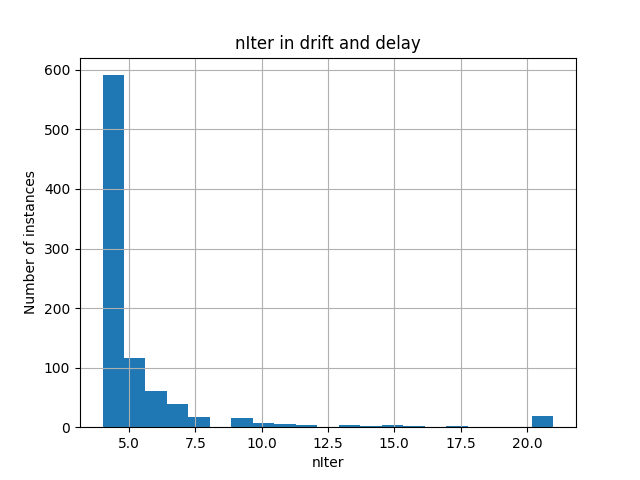
\includegraphics[width=\linewidth]{thesis/picture/heuristic/nIter_histogram_DD.png}
        \caption{Total iterations with delayed flights}
        \label{fig:heurDD:nIter}
    \end{subfigure}
    \hfill
    \begin{subfigure}{0.3\textwidth}
        \centering
        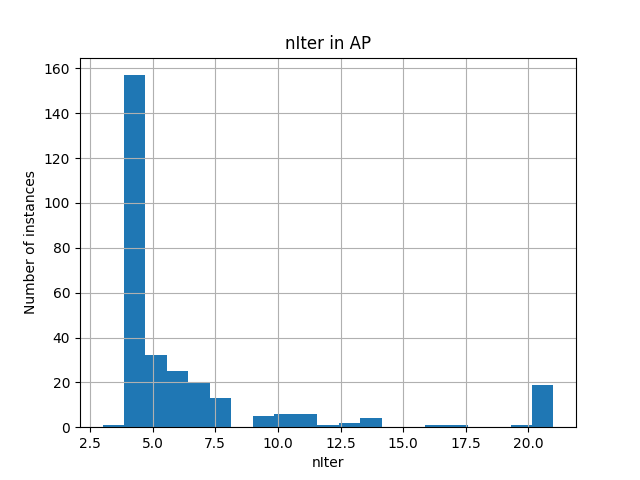
\includegraphics[width=\linewidth]{thesis/picture/heuristic/nIter_histogram_AP.png}
        \caption{Total iterations with high-priority flights}
        \label{fig:heurAP:nIter}
    \end{subfigure}
    \hfill
    \begin{subfigure}{0.3\textwidth}
        \centering
        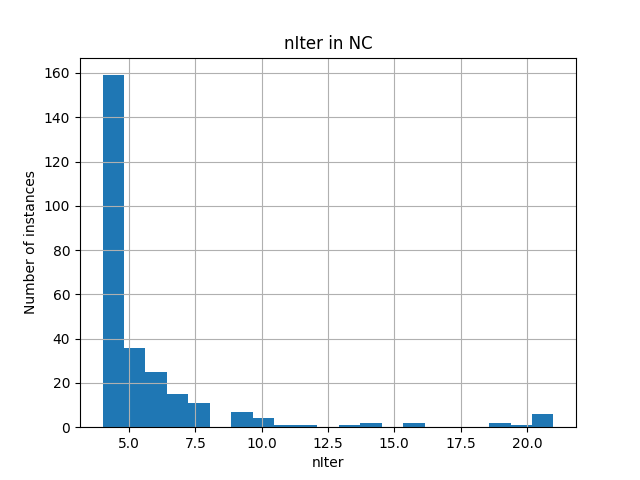
\includegraphics[width=\linewidth]{thesis/picture/heuristic/nIter_histogram_NC.png}
        \caption{Total iterations with non-collaborative intruder flights}
        \label{fig:heurNC:nIter}
    \end{subfigure}
    \caption{Total number of iterations needed to complete the heuristic}
    \label{fig:heur:nIter}
\end{figure}

\begin{figure}[ht]
    \centering
    \begin{subfigure}{0.3\textwidth}
        \centering
        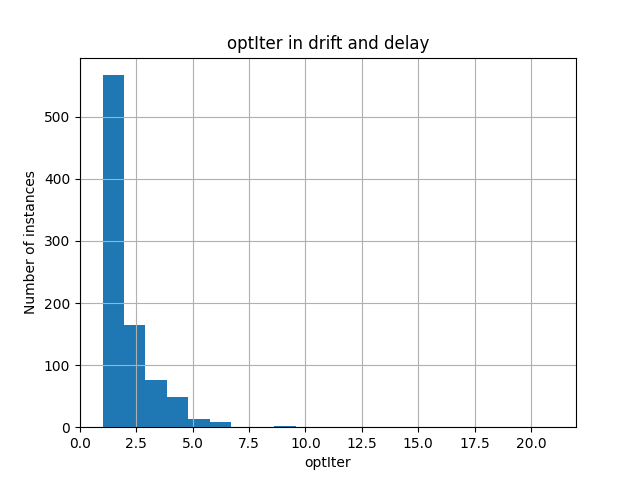
\includegraphics[width=\linewidth]{thesis/picture/heuristic/optIter_histogram_DD.png}
        \caption{Optimal iterations with delayed flights}
        \label{fig:heurDD:optIter}
    \end{subfigure}
    \hfill
    \begin{subfigure}{0.3\textwidth}
        \centering
        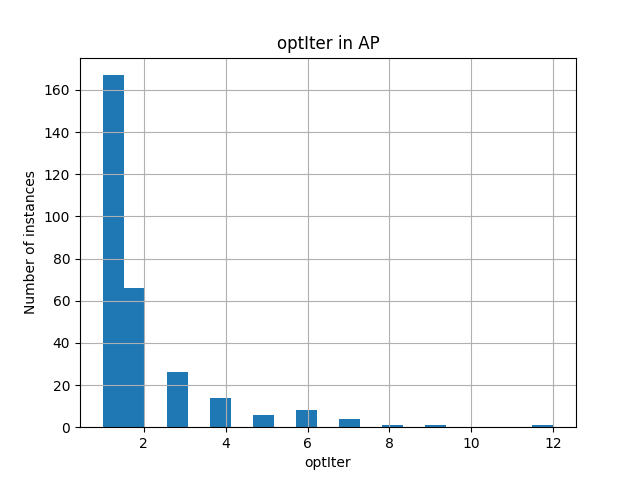
\includegraphics[width=\linewidth]{thesis/picture/heuristic/optIter_histogram_AP.png}
        \caption{Optimal iterations with high-priority flights}
        \label{fig:heurAP:optIter}
    \end{subfigure}
    \hfill
    \begin{subfigure}{0.3\textwidth}
        \centering
        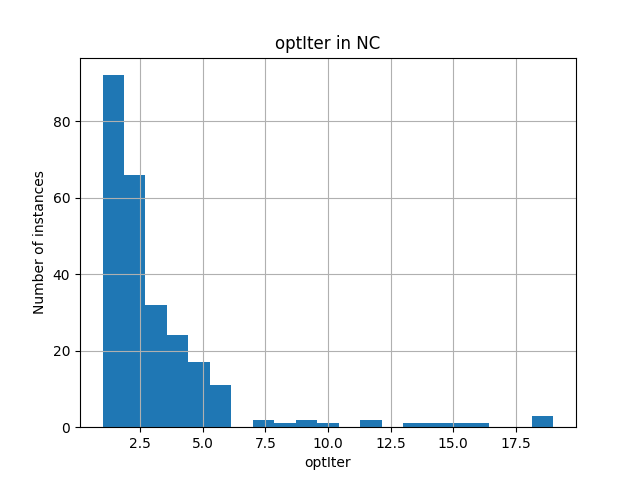
\includegraphics[width=\linewidth]{thesis/picture/heuristic/optIter_histogram_NC.png}
        \caption{Optimal iterations with non-collaborative intruder flights}
        \label{fig:heurNC:optIter}
    \end{subfigure}
    \caption{Number of iterations required to find the best heuristic solution}
    \label{fig:heur:optIter}
\end{figure}

{\tiny
\begin{longtable}{|l|r|r|r|r|r|r|}
\caption{Instances with extended time limit} \label{table:heuristic:overTimeLimit} \\ \hline
Instance & Time Limit& Optimal Value & Total Time & Time Best Solution & Num. Iterations & Optimal Iteration \\ \hline
\endfirsthead
\caption[]{Instances with extended time limit (continued)} \\ \hline
Instance & Time Limit& Optimal Value & Total Time& Time Best Solution & Num. Iterations & Optimal Iteration \\ \hline
\endhead
\multicolumn{7}{r}{Continued on next page} \\ \hline
\endfoot
\endlastfoot
metroplex53nDr0nDe2 & 240 & 21.418546 & 358.795575 & 358.723880 & 6 & 6 \\ \hline
metroplex63nDr0nDe3 & 360 & 458.553864 & 1436.318366 & 1436.271662 & 21 & 21 \\ \hline
\end{longtable}
}

\end{document}
